\section{Identifikation der Chl-Kataboliten des Brokkoliblattes mit MS Leafspray}

Im Folgenden werden die \gls{Chl-K}en beschrieben, die sich durch MS Leafspray identifizieren ließen. Die Strukturvorschläge wurden mit einem hochauflösenden Massenspektrometer überprüft (Kapitel \ref{sec:ChlKatabolitenBrokkoli} und \ref{sec:ChlKatabolitenESIMS}). Sie beruhen auf den exakten Molekülmassen und den daraus errechneten möglichen Summenformeln.

Fragmentierungsdiagramme wurden wie in Kapitel \ref{sec:fragmentierungsdiagramme} beschrieben erstellt.

\subsection{Bo-NCC-1} \label{sec:MSLeafsprayBoNCC1}

Bei diesem Kataboliten handelt es sich vermutlich um denselben, wie er auch in der Brokkolifrucht gefunden wurde, weswegen er die Bezeichnugn \textit{Bo}-NCC-1 erhält. \cite{ChlorophyllCatabolitesBroccoli} Beobachtet wurde die protonierte Verbindung bei m/z = 793 [M+H]\textsuperscript{+} und das Kaliumsalz bei m/z = 831 [M+K]\textsuperscript{+} (Abbildung \ref{fig:831MKLeafspray}). Aufgrund der geringen Intensitäten der protonierten Verbindung war es nicht möglich, ein verwertbares Massenspektrum dieser aufzunehmen. \\

Der Katabolit bei m/z = 831 [M+K]\textsuperscript{+} zeigte Abspaltungen von \ch{H2O} bei m/z = 813 [M - \ch{H2O} + K]\textsuperscript{+}, von \ch{CO2} bei m/z = 787 [M - \ch{CO2} + K]\textsuperscript{+} und eine Folge von Abspaltungen bei m/z = 311 [M - (Ring A, Zucker, Ring D, \ch{CO2}) + K]\textsuperscript{+} (Begründung der Zuordnung siehe Kapitel \ref{sec:ChlKatabolitenESIMS}). Die Abspaltungen bei m/z = 798 [M - (\gls{nAb}) + K]\textsuperscript{+}, m/z = 586 [M - (\gls{nAb}) + K]\textsuperscript{+} und m/z = 551 [M - (\gls{nAb}) + K]\textsuperscript{+} können nicht eindeutig zugeordnet werden, da hierzu weitere experimentelle Daten und die exakten Molekülmassen notwendig sind. 

\begin{figure}[!htbp]
  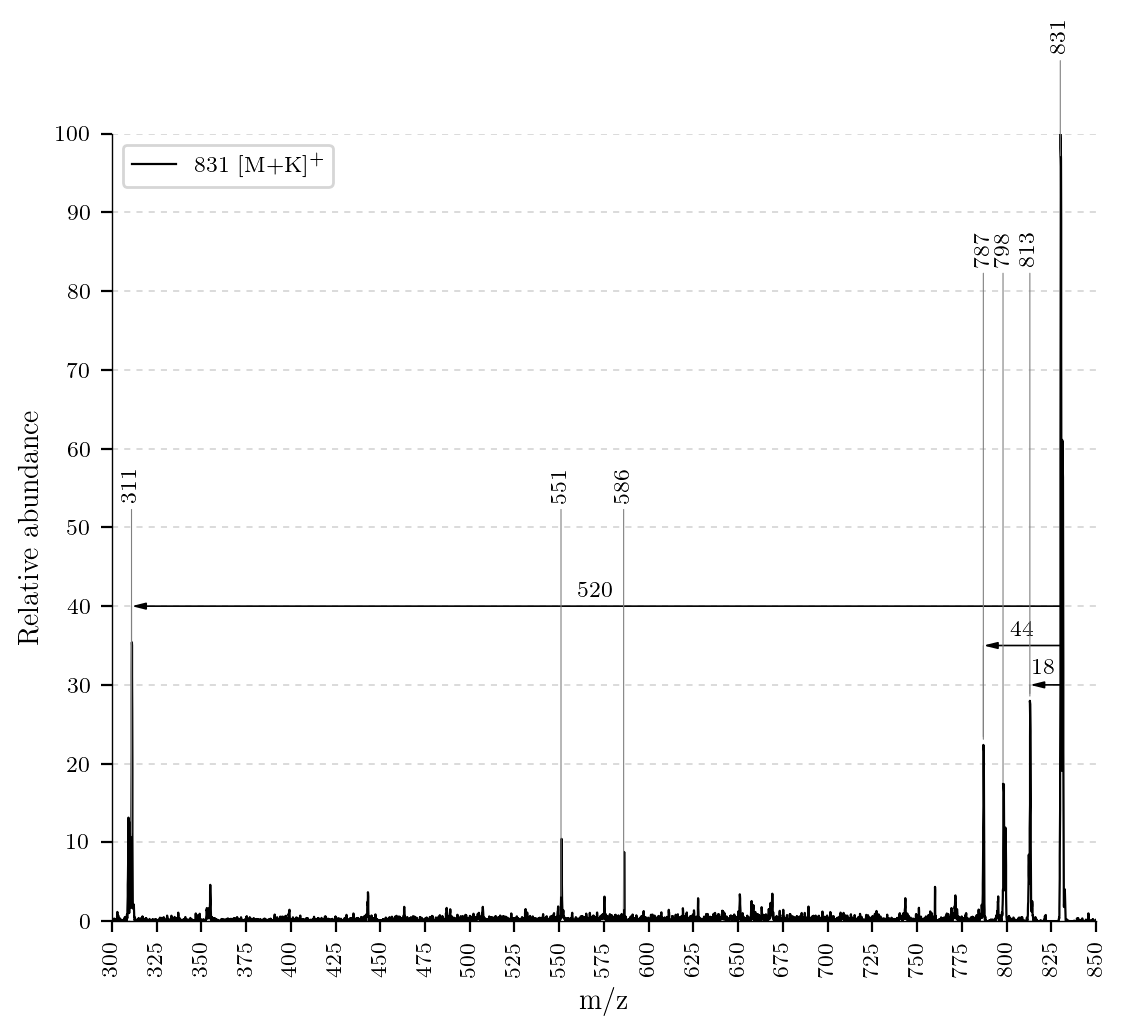
\includegraphics[width=\textwidth, height=0.7\textwidth]{figures/Kapitel4/Kataboliten/VWA_MS_LeafSpray_831.png}
  \caption[ESI-MS Spektrum von \textit{Bo}-NCC-1, Quelle: Autor]{ESI-MS von \textit{Bo}-NCC-1 mit m/z = 831 [M+K]\textsuperscript{+}}
  \label{fig:831MKLeafspray}
\end{figure}

Das Fragment bei m/z = 798 [M - (\gls{meoh}?) + K]\textsuperscript{+} ist insofern interessant, da es sich hierbei um eine Abspaltung von \gls{meoh} (-32 Da) handeln könnte, was aber nicht mit der Struktur des \textit{Bo}-NCC-1 (Abbildung \ref{fig:831MKLeafspraystructure}) vereinbar wäre. Die Frage, ob es sich bei der Abweichung von einem Da um eine Ungenauigkeit des Massenspektrometers handelt oder ob doch ein anderes Fragment abgespalten wird, bleibt offen, weswegen auf diese Abspaltung in den weiteren Ausführungen nicht näher eingegangen.

Wie aus dem Fragmentierungsdiagramm (Abbildung \ref{fig:831MKLeafspraydiags}) ersichtlich, erfolgt die Abspaltung von \ch{H2O} bei einer niedrigeren \gls{nKE} wie jene von \ch{CO2} und verschwindet bei höheren Energien, wohingegen die Abspaltung von \ch{CO2} erhalten bleibt. Die Abspaltung von \ch{H2O} erreicht ein lokales Maximum bei einer \gls{nKE} von 10. Die Abspaltung von \ch{CO2} erreicht ein lokales Maximum bei 30 \gls{nKE}.

Aufgrund der \ch{CO2} Abspaltung wird an Position C-8\textsuperscript{2} eine Carbonsäuregruppe vermutet (wie in \cite{StructureElucidation} gezeigt), die über einen Mechanismus wie unter anderem in Abbildung \ref{fig:619MHElectronMovement} vorgeschlagen, abgespalten wird. Die relativ große Molekülmasse weist zudem auf einen Zucker an Position C-3\textsuperscript{2} hin. Die Summenformel des \textit{Bo}-NCC-1 konnte über die exakte Molekülmasse mit einem hochauflösenden Massenspektrometer bestimmt werden (Kapitel \ref{sec:ESIMSBoNCC1}).

\begin{figure}[!htbp]
  \begin{subfigure}[b]{0.5\textwidth}
    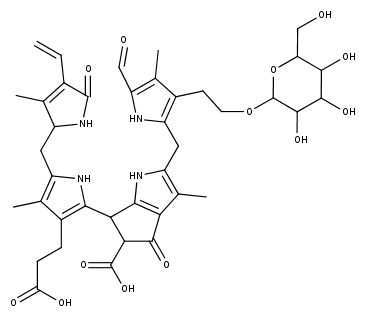
\includegraphics[width=\textwidth]{figures/Kapitel4/Kataboliten/fragmentation_structures/VWA_Katabolit_831.png}
    \caption{}
    \label{fig:831MKLeafspraystructure}
  \end{subfigure}
  \hfill
  \begin{subfigure}[b]{0.7\textwidth}
    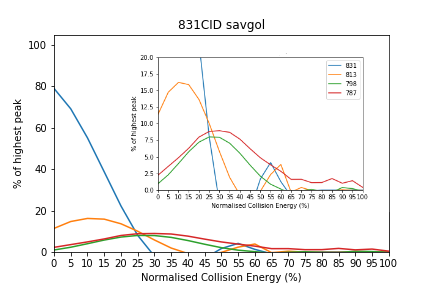
\includegraphics[width=\textwidth]{figures/Kapitel4/Kataboliten/diags/831CID-savgol.png}
    \caption{}
    \label{fig:831MKLeafspraydiags}
  \end{subfigure}
  \caption[Strukturvorschlag von \textit{Bo}-NCC-1 und Fragmentierungsdiagramm, Quelle: Autor]{(a) Strukturvorschlag des \textit{Bo}-NCC-1 mit Summenformel \ch{C40H48N4O13}, (b) Fragmentierungsdiagramm von \textit{Bo}-NCC-1 (blau = 831 [M+K]\textsuperscript{+}, orange = 813 [M - \ch{H2O} + K]\textsuperscript{+}, grün = 798 [M - (\ch{MeOH} - \gls{nAb}) + K]\textsuperscript{+}, rot = 787 [M - \ch{CO2} + K]\textsuperscript{+})}
\end{figure}



\subsection{Bo-NCC-3}

Beim \textit{Bo}-NCC-3 handelt es sich um einen \gls{Chl-K}en, der bisher nicht in der Brokkolifrucht identifiziert wurde \cite{ChlorophyllCatabolitesBroccoli}, weswegen er als dritter, in der Brokkolipflanze gefundener Katabolit den Index 3 erhält. Analysiert wurde das Kaliumsalz mit m/z = 685 [M+K]\textsuperscript{+}. \\

Es wurden zwei charakteristische Abspaltungen von \ch{H2O} bei m/z = 667 [M - \ch{H2O} + K]\textsuperscript{+} sowie von \ch{CO2} bei m/z = 641 [M - \ch{CO2} + K]\textsuperscript{+} beobachtet. Bei den Abspaltungen bei m/z = 429 [M - (\gls{nAb}) + K]\textsuperscript{+}, m/z = 561 [M - (\gls{nAb}) + K]\textsuperscript{+}, m/z = 605 [M - (\gls{nAb}) + K]\textsuperscript{+} und m/z = 652 [M - (\gls{nAb}) + K]\textsuperscript{+} ist nicht eindeutig geklärt, welche Fragmente hierbei entstanden sind. Für das Fragment bei m/z = 652 [M - (\gls{meoh}?) + K]\textsuperscript{+} gilt dasselbe wie bei der Abspaltung von m/z = 798 [M - (\ch{MeOH}?) + K]\textsuperscript{+} von \textit{Bo}-NCC-1 (Kapitel \ref{sec:MSLeafsprayBoNCC1}). Um diese Fragmente aufzuklären, müssten weitere Experimente des Kaliumsalzes mit einem hochauflösenden Massenspektrometer durchgeführt werden. Fragmentierungen der protonierten Verbindung konnten mit einem hochauflösenden Massenspektrometer gemessen werden (Kapitel \ref{sec:ESIMSBoNCC3}).

\begin{figure}[htbp]
  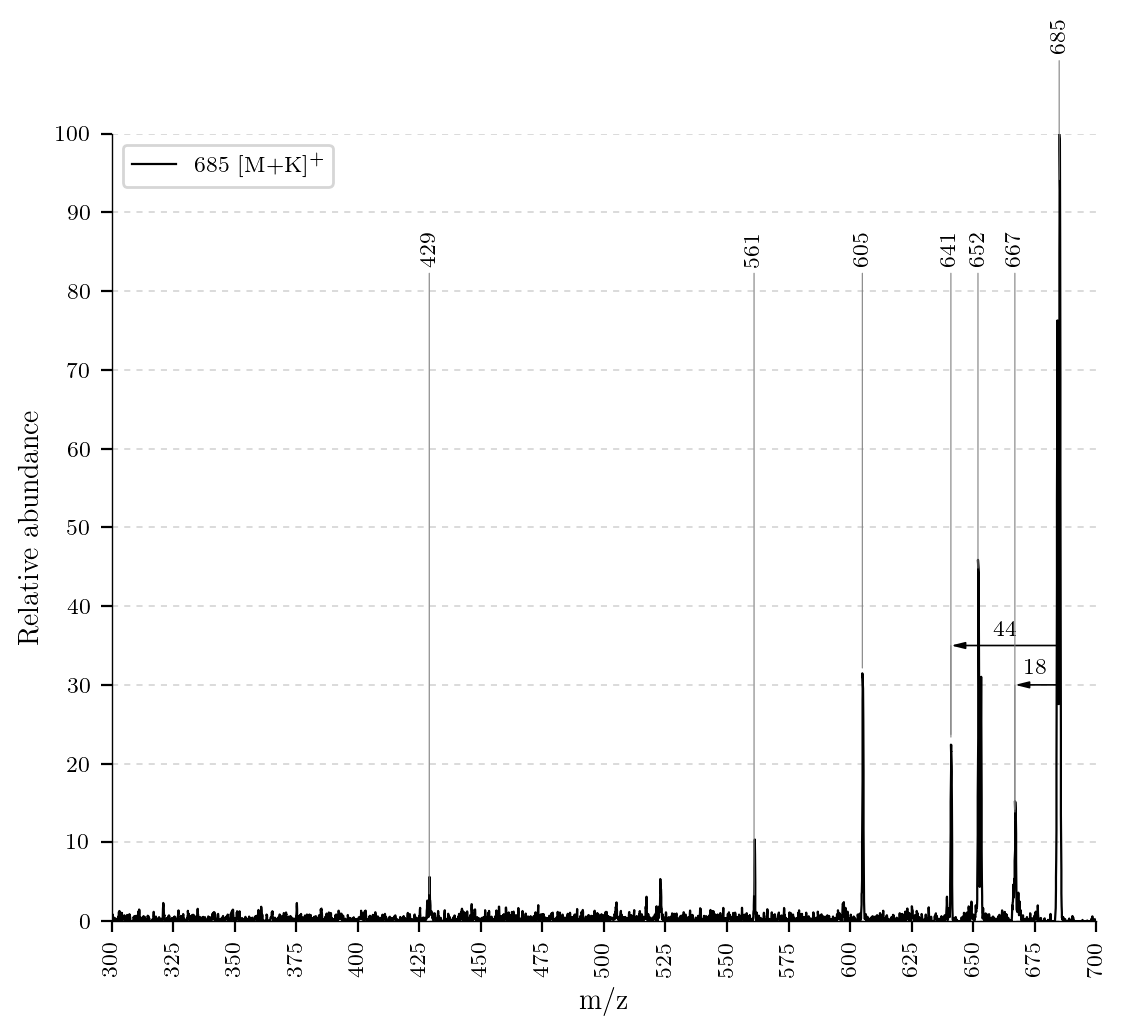
\includegraphics[width=\textwidth, height=0.7\textwidth]{figures/Kapitel4/Kataboliten/VWA_MS_LeafSpray_685.png}
  \label{fig:685MKLeafspray}
  
  \caption[ESI-MS von \textit{Bo}-NCC-3, Quelle: Autor]{ESI-MS von \textit{Bo}-NCC-3 mit m/z = 685 [M+K]\textsuperscript{+}}
\end{figure}

\begin{figure}[!htbp]
  \begin{subfigure}[b]{0.4\textwidth}
    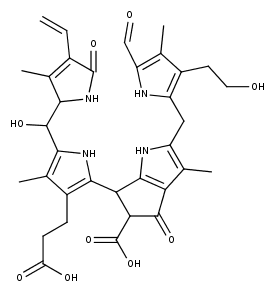
\includegraphics[width=\textwidth]{figures/Kapitel4/Kataboliten/fragmentation_structures/VWA_Katabolit_685.png}
    \caption{}
    \label{fig:685MKLeafspraystructure}
  \end{subfigure}
  \hfill
  \begin{subfigure}[b]{0.7\textwidth}
    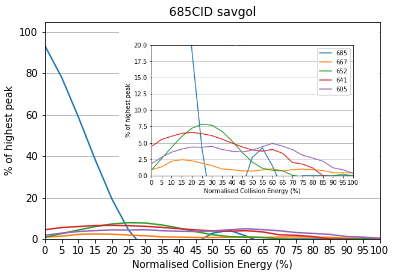
\includegraphics[width=\textwidth]{figures/Kapitel4/Kataboliten/diags/685CID-savgol.png}
    \caption{}
    \label{fig:685MKLeafspraydiags}
  \end{subfigure}
  \caption[Strukturvorschlag von \textit{Bo}-NCC-3 und Fragmentierungsdiagramm, Quelle: Autor]{(a) Strukturvorschlag von \textit{Bo}-NCC-3 mit Summenformel \ch{C34H38N4O9}, (b) Fragmentierungsdiagramm von \textit{Bo}-NCC-3 (blau = 685 [M+K]\textsuperscript{+}, orange = 667 [M - \ch{H2O} + K]\textsuperscript{+}, grün = 652 [M - (\gls{meoh}?) + K]\textsuperscript{+}, rot = 641 [M - \ch{CO2} + K]\textsuperscript{+}, violett = 605 [M - (\gls{nAb}) + K]\textsuperscript{+})}
\end{figure}

Das Fragmentierungsdiagramm zeigt, dass die Abspaltung von \ch{H2O} bei einer niedrigeren \gls{nKE} erfolgt, wie jene von \ch{CO2}, da sie ihre höchste Intensität zuvor erreicht (bei einer \gls{nKE} von 15 - \ch{H2O} im Vergleich zu 20 - \ch{CO2}). 

Im Vergleich zum \textit{Bo}-NCC-1 zeigt der Graph ein lokales Maximum der \ch{H2O} Abspaltung bei höheren Energien (beim \textit{Bo}-NCC-3 bei 15 \gls{nKE} wohingegen beim \textit{Bo}-NCC-1 bereits bei 10 \gls{nKE}). Das lokale Maximum der \ch{CO2} Abspaltung verschiebt sich von 30 \gls{nKE} beim \textit{Bo}-NCC-1 auf 20 \gls{nKE} beim \textit{Bo}-NCC-3. Das lokale Maximum der potentiellen Abspaltung von \gls{meoh} würde sich von 25 \gls{nKE} beim \textit{Bo}-NCC-1 auf 30 \gls{nKE} beim \textit{Bo}-NCC-3 verschieben (Abbildungen \ref{fig:831MKLeafspraydiags} und \ref{fig:685MKLeafspraydiags}).\\ 

Wie beim Bo-NCC-1 weist die \ch{CO2} Abspaltung auf eine freie Carbonsäure an Position C-8\textsuperscript{2} hin. Aufgrund der durch die Summenformel erhaltenen Sauerstoffanzahl wird angenommen, dass sich an Position C-15 eine Hydroxygruppe befindet (Abbildung \ref{fig:685MKLeafspraystructure}). Es wird vermutet, dass es sich dabei um eine Vorstufe zu einem \gls{YCC} handelt. [Referenz]

\subsection{Bo-DNCC}

Es wird vermutet, dass der \textit{Bo}-DNCC des Brokkoliblattes ident ist mit dem \textit{Bo}-DNCC der Brokkolifrucht. \cite{ChlorophyllCatabolitesBroccoli} Beobachtet wurden zwei Pseudo-Molekulare Ionen. Eines mit m/z = 619 [M+H]\textsuperscript{+} (Abbildung \ref{fig:619MHLeafspray}) und mit m/z = 657 [M+K]\textsuperscript{+} (Abbildung \ref{fig:657MKLeafspray}).\\

Der Katabolit bei m/z = 619 [M+H]\textsuperscript{+} zeigte Abspaltungen von \ch{H2O} bei m/z = 601 [M - \ch{H2O} + H]\textsuperscript{+}, von \ch{CO2} bei m/z = 575 [M - \ch{H2O} + H]\textsuperscript{+}, von Ring D (zusammen mit einer Abspaltung von \ch{CO2}) bei m/z = 452 [M - (Ring D, \ch{CO2}) + H]\textsuperscript{+} und von Ring A, Ring D und \ch{CO2} bei m/z = 311 [M - (Ring A, Ring D, \ch{CO2}) + H]\textsuperscript{+} (Abbildung \ref{fig:619MHLeafspray} - Zuordnung Kapitel \ref{sec:ESIMSBoDNCC}).

\begin{figure}[!htbp]
  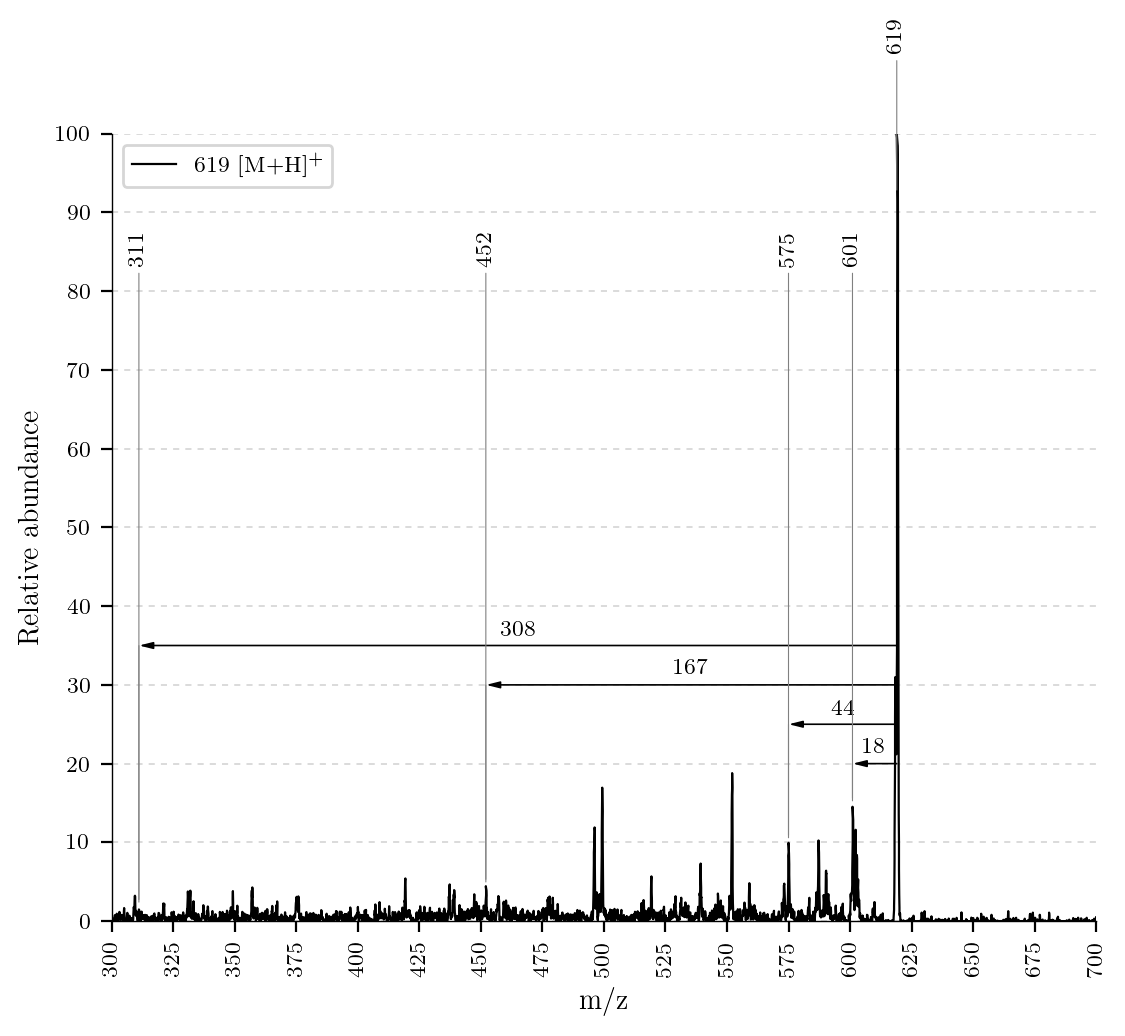
\includegraphics[width=\textwidth, height=0.7\textwidth]{figures/Kapitel4/Kataboliten/VWA_MS_LeafSpray_619.png}
  \caption[ESI-MS von \textit{Bo}-DNCC, Quelle: Autor]{ESI-MS von \textit{Bo}-DNCC bei m/z = 619 [M+H]\textsuperscript{+}}
  \label{fig:619MHLeafspray}
\end{figure}

Das Kaliumsalz des \textit{Bo}-DNCC mit m/z = 657 [M+K]\textsuperscript{+} zeigte eindeutige Abspaltungen von \ch{H2O} bei m/z = 639 [M - \ch{H2O} + K]\textsuperscript{+} und von \ch{CO2} bei m/z = 613 [M - \ch{CO2} + K]\textsuperscript{+} (Abbildung \ref{fig:657MKLeafspray}). Die Abspaltungen bei m/z = 375 [M - (\gls{nAb}) + K]\textsuperscript{+} und m/z = 577 [M - (\gls{nAb}) + K]\textsuperscript{+} können nicht eindeutig zugeordnet werden.

\begin{figure}[!htbp]
  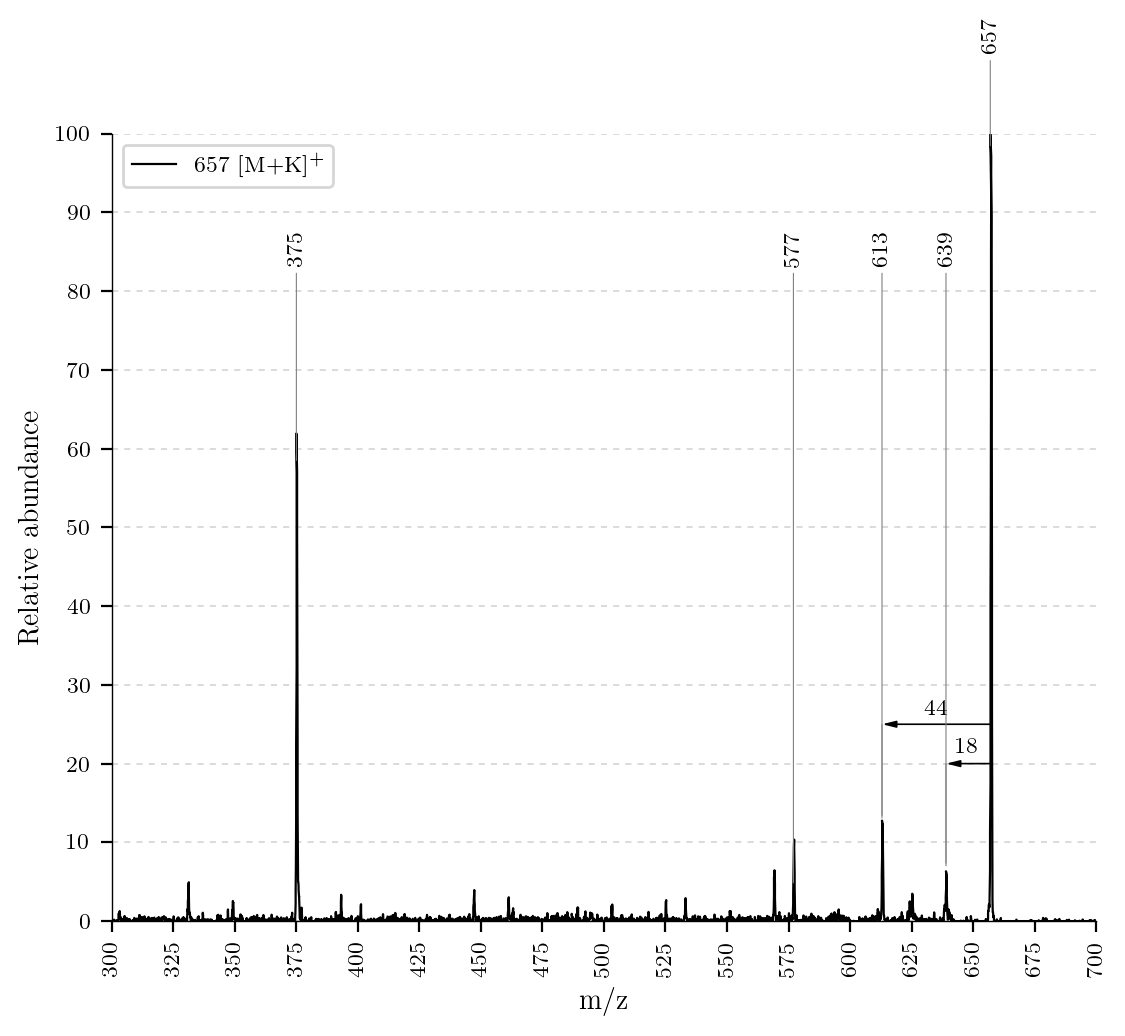
\includegraphics[width=\textwidth, height=0.7\textwidth]{figures/Kapitel4/Kataboliten/VWA_MS_LeafSpray_657.png}
  \caption[ESI-MS von \textit{Bo}-DNCC, Quelle: Autor]{ESI-MS von \textit{Bo}-DNCC bei m/z = 657 [M+K]\textsuperscript{+}}
  \label{fig:657MKLeafspray}
\end{figure}

\begin{figure}[!htbp]
  \begin{subfigure}[b]{0.4\textwidth}
    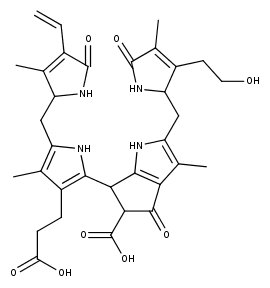
\includegraphics[width=\textwidth]{figures/Kapitel4/Kataboliten/fragmentation_structures/VWA_Katabolit_619.png}
    \caption{}
    \label{fig:619MKLeafspraystructure}
  \end{subfigure}
  \hfill
  \begin{subfigure}[b]{0.7\textwidth}
    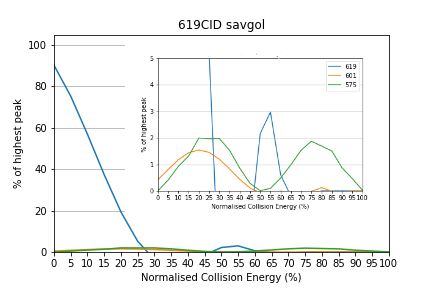
\includegraphics[width=\textwidth]{figures/Kapitel4/Kataboliten/diags/619CID-savgol.png}
    \caption{}
    \label{fig:619MKLeafspraydiags}
  \end{subfigure}
  \caption[Strukturvorschlag von \textit{Bo}-DNCC mit Fragmentierungsdiagramm, Quelle: Autor]{(a) Strukturvorschlag von \textit{Bo}-DNCC mit Summenformel \ch{C33H38N4O8}, (b) Fragmentierungsdiagramm von \textit{Bo}-DNCC (blau = 619 [M+H]\textsuperscript{+}, orange = 601 [M - \ch{H2O} + H]\textsuperscript{+}, grün = 575 [M - \ch{CO2} + H]\textsuperscript{+})}
\end{figure}

Die \ch{H2O} Abspaltung beim \textit{Bo}-DNCC erreicht ein lokales Maximum bei 20 \gls{nKE} und erfolgt damit im Vergleich zum Bo-NCC-1 und Bo-NCC-3 bei der höchsten \gls{nKE}. Die Abspaltung von \ch{CO2} weist beim \textit{Bo}-DNCC zwei lokale Maxima, bei 25 \gls{nKE} und 75 \gls{nKE} auf. Das lokale Maximum an der Stelle 75 \gls{nKE} ist dabei etwas weniger intensiv ausgeprägt wie jenes an der Stelle 25 \gls{nKE}. Das erste lokale Maximum befindet sich damit an der gleichen Stelle wie beim \textit{Bo}-NCC-1 und \textit{Bo}-NCC-3 (Abbildungen \ref{fig:831MKLeafspraydiags} und \ref{fig:685MKLeafspraydiags}). Das zweite Maximum kann noch nicht geklärt werden, da es bei den anderen bisher analysierten Kataboliten nicht beobachtet wurde.

Es ist fraglich, ob der Vergleich mit den Fragmentierungsdiagrammen von \textit{Bo}-NCC-1 und \textit{Bo}-NCC-3 möglich ist, da bei diesen das [M+K]\textsuperscript{+} Ion aufgenommen wurde.
